%%%%%%%%%%%%%%%%%%%%% chapter.tex %%%%%%%%%%%%%%%%%%%%%%%%%%%%%%%%%
%
% sample chapter
%
% Use this file as a template for your own input.
%
%%%%%%%%%%%%%%%%%%%%%%%% Springer-Verlag %%%%%%%%%%%%%%%%%%%%%%%%%%

\chapstarthook{El contenido de este ap�ndice ha sido enviado a \emph{Journal of Web Engineering (JWE)}}

\chapter{Requirements in Web engineering: a systematic literature review.}
\label{a1} % Always give a unique label
% use \chaptermark{}
% to alter or adjust the chapter heading in the running head

\chaptermark{Requirements engineering in Web: a systematic literature review}

\begin{figure}[h!]
  \begin{center}
    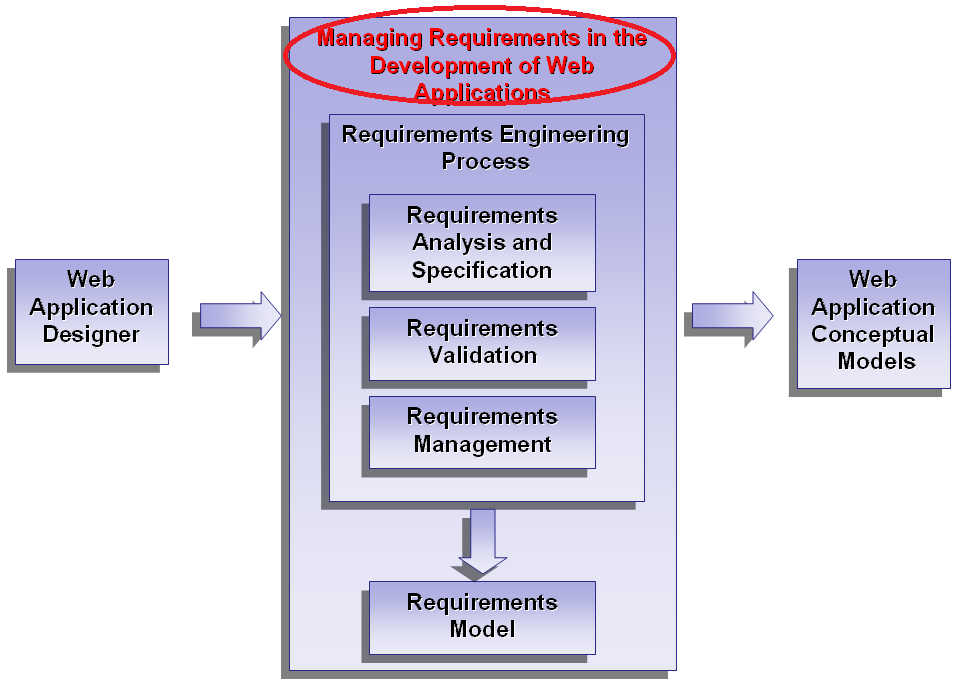
\includegraphics[width=0.7\textwidth]{img/PropuestaCapSLR.png}
  \end{center}
  %\caption{} \label{}
\end{figure}


El art�culo presentado en este ap�ndice es una extensi�n del Cap�tulo~\ref{c3} de la tesis doctoral en el que se destaca la importancia de considerar a los requisitos en el desarrollo de sistemas Web. En particular, en la revisi�n sistem�tica de la literatura presentada en el ap�ndice, se ha mejorado el trabajo descrito en el Cap�tulo~\ref{c3} de la siguiente forma:

\begin{itemize}
	\item La estrategia de b�squeda ha sido mejorada, por lo tanto se han a�adido m�s m�todos
a la revisi�n.

\item El estudio se ha centrado en analizar el proceso de ingenier�a de requisitos en el desarrollo de aplicaciones Web, es decir, en qu� forma los requisitos son tratados en lo que respecta al an�lisis, especificaci�n, validaci�n y la gesti�n de los mismos. 

\item La revisi�n sistem�tica analiza el vocabulario que ha sido adoptado por cada 
m�todo de ingenier�a Web de una manera met�dica y completa mediante el uso de la clasificaci�n propuesta por Escalona y Koch \cite{EscalonaK04}.
\end{itemize}

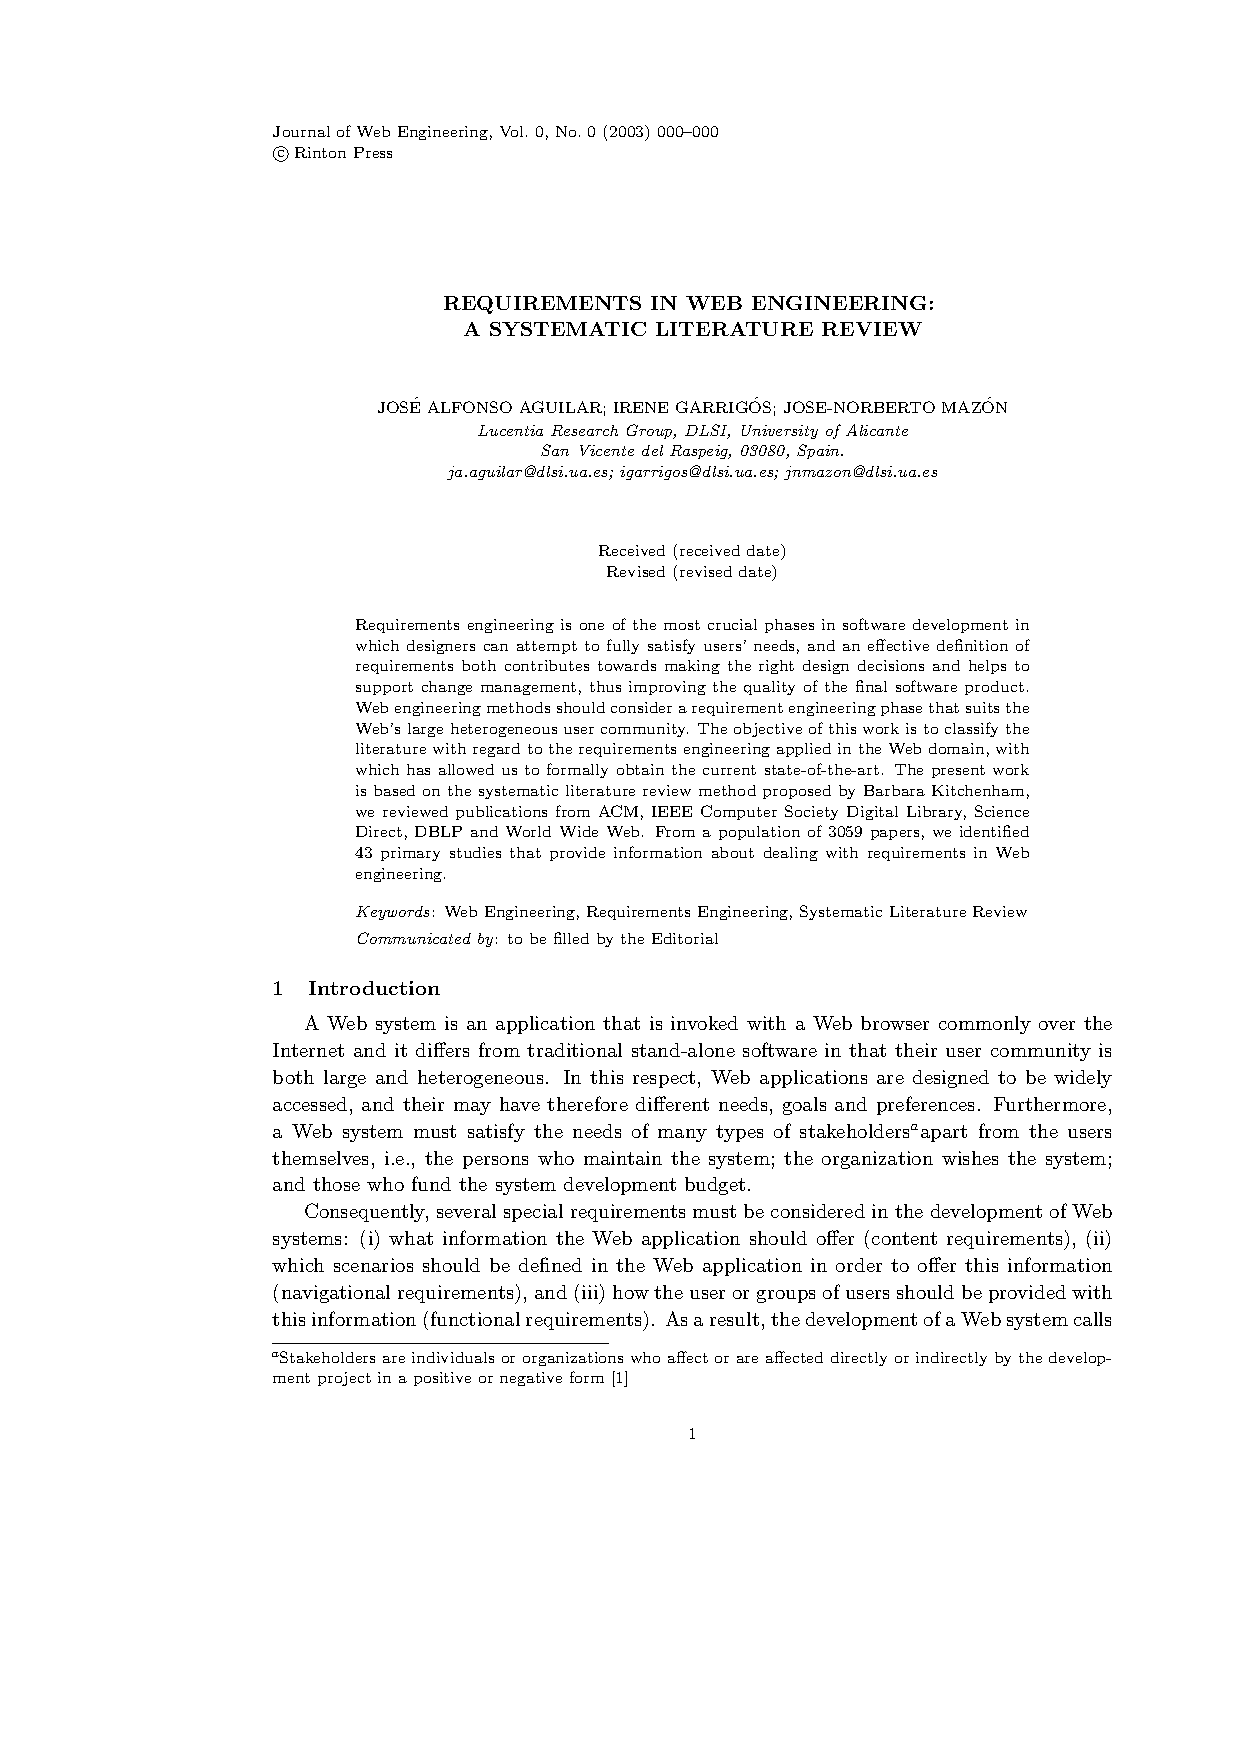
\includepdf[openright=true,pages={1-31}]{papers/apendice/AguilarJWE2011_Final.pdf}